\section{Skin recognition}
    Liveness detection motivations.

    Fast face detection motivations.

    \subsection{How it works?}
        Wide description about material detection
        with light reflectiveness.

    \subsection{Technical aspect -- how camera works?}
        To think about security aspect of skin detection,
        it's critical to understand how image sensors works.
        Most common are \textit{CCD} (\textit{charge-coupled device})
        and \textit{CMOS} (\textit{complementary metal-oxide-semiconductor})
        [TODO: LINK NEEDED]. % Most common?
        Due to better quality, as well as sensitiveness, for security reasons
        it probably would be better to use CCD.
        However, both matrices have same problem -- limitation on wavelength sensitivity.
        Such sensors are sensitive to wavelengths aproximetly up to 1050nm,
        which may be serious limitation as skin ligthen with greater wavelength has
        more undifferentiated characteristics.
        Therefore looking for best possible skin detection method,
        it may be convenient to assume that other type of light sensitive matrices
        are in reach of inventor.
        Nevertheless we were limited to very common cameras.

        TODO: Paragraph about light sensors materials and other types of image sensors.
        Paragraph under maintenance. May dissapear.

        We are describeing one possible realization, keep in mind that
        there are more solutions than that, but we don't find them usfeful in our problem.

        \subsubsection*{Monochrome}
            As image sensor is matrix build from many small photodiodes,
            % TODO: in fact working like...
            it's natural to create monochromatic image.
            Because photodiodes don't distinguish different
            wavelength, only light intensity, it's hard
            to measure light reflectiveness.
            The only possible way to do that is to
            make different picture for every wavelength.
            It's not easy, as you have to
            provide your own lighting and somehow remove
            light coming from other sources.
            Also, all pictures have to be made in
            a~very short time interval, as the subject
            cannot move between shots.

        \subsubsection*{Multispectral imaging}
            Multispectral imaging is answer to
            problem of object's move,
            way to measure every wavelength intensity in one picture.
            Probably easies way to describe it is to look at RGB camera.
            There every photodiode is responsible for exacly one colour,
            where as colour we understand wavelength interval (it's important
            to understand, that we can consider any wavelength interval as one colour).
            And result picture is built from small squares (mostly $2 \times 2$)
            of photodiode matrix data.
            There may be more than just  three colours in fact.
            For example, you may find camera which see two types of ''green''.
            Mostly, at the end everything is converted to known RGB format.

            \begin{center}
                \includegraphics{RGB-matrix}
            \end{center}

            Software receives from camera imformation with light intensity at every
            sensor and information which colour it sees.

            One from possible realisations of reducing the range
            of light visible through the sensor is to take standard image sensor which
            may see full specturm of light ($350$-$1050$nm.) and
            place filters in way that only specific light will reach choosen photodiode.

            \begin{center}
                \includegraphics[scale=0.40]{RGB-filter}
            \end{center}

        \subsubsection*{Hyperspectral imaging}
            Hyperspectral imaging is creating pictures using camera with
            capabilityy to distinguish many and many of colours (more like hundreds or thousands)
            instead of just few.
            It would be very helpful, obviously, in skin-detection device,
            but there is very little chance to see such device in mobile phones soon.

    \subsection{Technical aspect -- how it may be created?}
        As we know how camera works, we can say that there are only two ways of
        building skin detection mobile device.
        \subsubsection*{Monochrome}
            We can work without filters (or with one for whole camera),
            but then we have to make picture for every wave lenght.
            Also, we need one diode with that very wavelength we want.
            It's easier method to build in phone, but taking pictures
            must be very fast.

            Bigest pros of that solution is possibility of lighting
            with different LEDs in random moment of time, so hackers
            will no be able to play with own diods to modify result.

        \subsubsection*{Multispectral imaging}
            Also there is possibility to use filters with specific infrared colours.
            But important here is avoiding standard smoothing algorithms used
            in cameras. We truly need real light intensity from every sensor.
            Not smoothed or reduced one.

    \subsection{Our attempts}

        \subsubsection{Detecting reflectiveness using Kinect}
            Our first idea was to use a Kinect v2 depth and infrared camera to detect
            how well does a surface reflect light.
            Kinect v2 cameras have their own source of infrared light and they make
            a very good job at filtering other sources of light.
            So, for each pixel on the infrared image, we know how much light coming
            from the Kinect's light emitter was reflected in that particular place.
            Also, Kinects are depth cameras, which additionally gives us the information
            on how far away from the camera is the object visible on that pixel.

            Since the source of light is in the same device as the camera, the distance
            seen on the depth image is also the distance from the light emitter.
            This is an important observation, because we know how distance affects how
            much light arrives at a particular place. % might need a better wording
            If we have a source of light that, at a given distance, lights up a
            1cm $\times$ 1cm square of a flat surface with a particular amount
            of light, then at double that distance it will light up a 2cm $\times$ 2cm
            square with the same amount of light, which means that the same amount
            of light is distributed over a 4 times larger surface, so the
            intensity of light has to be 4 times lower than before.

            With those observations, we took pairs of IR and depth images, and for each
            pixel calculated a new value of $ir-intensity \cdot depth \cdot depth$,
            which should estimate how well light was reflected at that point,
            regardless of distance from the camera.

            \begin{figure}[H]
                \caption{An unprocessed IR photo, and an image calculated using
                the method described above.}
                \centering
                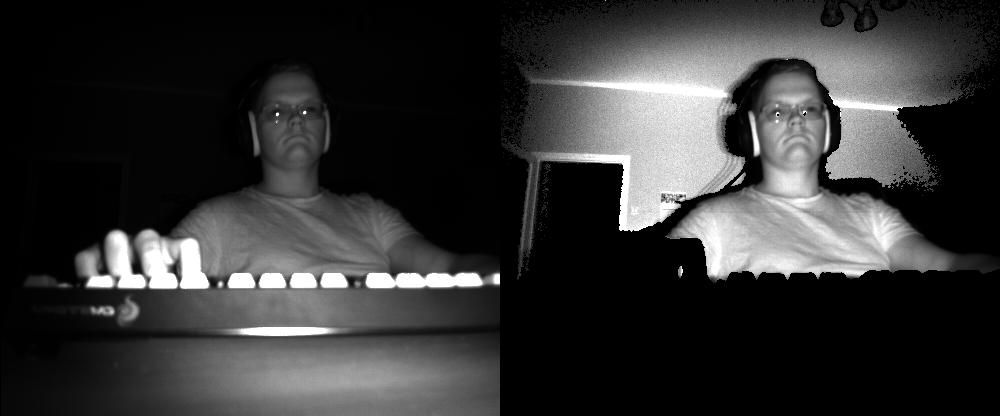
\includegraphics[width=\textwidth]{skin_kinect_1}
                \label{fig:skin_kinect_1}
            \end{figure}

            As seen on figure \ref{fig:skin_kinect_1}, we have accidentally created
            a night vision camera (please note that some of the black areas are there because Kinect cameras do not give depth data for objects closer than 50cm)
            -- but this means that our idea is to some extent working, because the point
            of it was to make objects in the distance indistinguishable from those close
            to the camera.

            However, one this that is not considered in that method is that objects
            can also be at different angles to the camera.
            A sheet of paper perpendicular to the source of light will reflect more
            light to the Kinect than it would reflect if it was at a 45 degrees angle.

            \begin{figure}[H]
                \caption{Three IR images processed with the described method, with a
                manually determined interval of values marked red.}
                \centering
                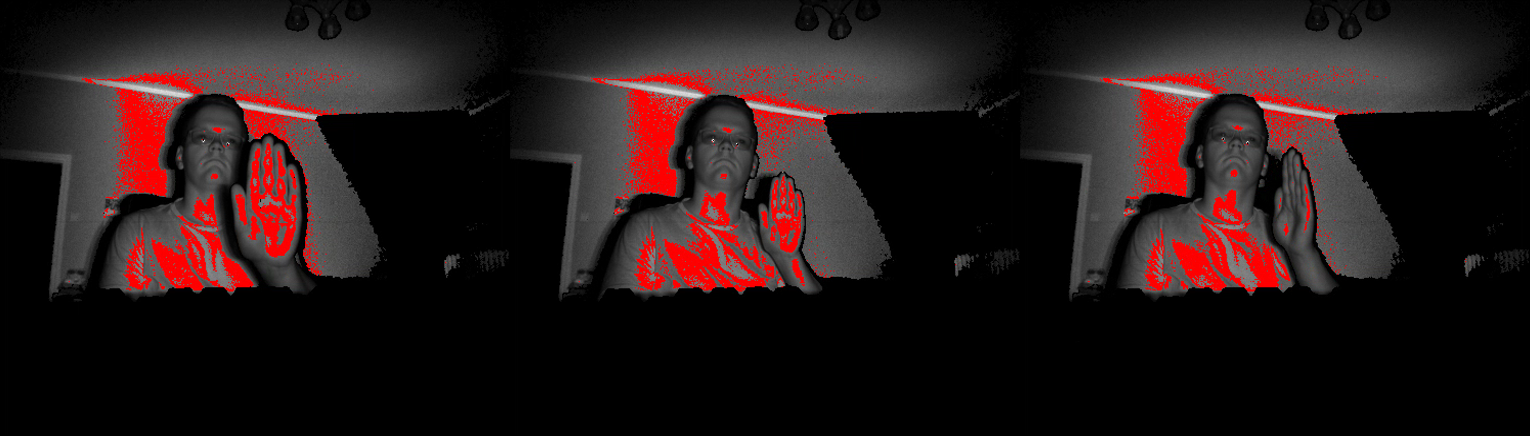
\includegraphics[width=\textwidth]{skin_kinect_2}
                \label{fig:skin_kinect_2}
            \end{figure}

            We have manually selected an interval of values and marked them red, which
            can be seen on figure \ref{fig:skin_kinect_2}.
            On the first two pictures there, the hand is at the same angle, but at a
            different distance to the camera.
            It is visible that the calculated values remained very close regardless
            of the distance, which was a success.
            However, on the third picture, the hand is at a different angle and
            that changes how it reflects light towards the camera, which makes the values
            different.

            Knowing the depth value and certain properties of the camera, it is possible
            to calculate the 3D coordinates of each pixel.
            With that information, it is possible to calculate the angle towards the
            camera between each two pixels, and then use that value in the method above
            to make it independent of angles.
            However, our attempts to do this were unsuccessful, possibly because the
            depth camera is not precise enough.
            % TODO Dominik: maybe describe briefly the mathematical details of what
            %               was attempted

        \subsubsection{Using three infrared wavelengths}
            \subsubsection*{Prototype}
            With the previous method using only one light wavelength (the one emitted by
            Kinect), we decided to take photos using three different wavelengths.
            This gives the opportunity to analyze how does the way the objects reflect
            light changes with regard to light wavelength, instead of directly looking
            at how bright a point is.

            To make any research, we had to take three photos of the same object
            reflecting three different wavelengths of infrared light.
            The camera, the infrared light sources, and the photographed object
            had to be in the same position for all of the photos.
            An ideal way to do this would be to use a spectral camera, but they are
            very expensive and we were not able to use one.

            One possible way to take a photo of how a certain wavelength is reflected
            would be to use a filter that only lets that wavelength to pass through it.
            However, changing filters on the camera between taking photos would take
            a lot of time, which would create a risk of changing the relative position
            of the object and the camera, which is unacceptable.

            We borrowed a mobile phone which had a filter mounted on its front camera
            that allowed various wavelengths of infrared light, but not visible light.
            This opened up the opportunity to take a different approach -- instead
            of filtering the selected wavelength, we want to illuminate the object
            using only that wavelength.

            We purchased diodes emitting light in the following wavelengths:
            850nm, 890nm, 940nm. Those diodes were connected to an Arduino board.
            We used two diodes of each wavelength, and mixed their positions to
            make sure that the centers of sources of light at each wavelength
            are as close as possible.

            \begin{figure}[H]
                \caption{Arduino board with six IR diodes.}
                \centering
                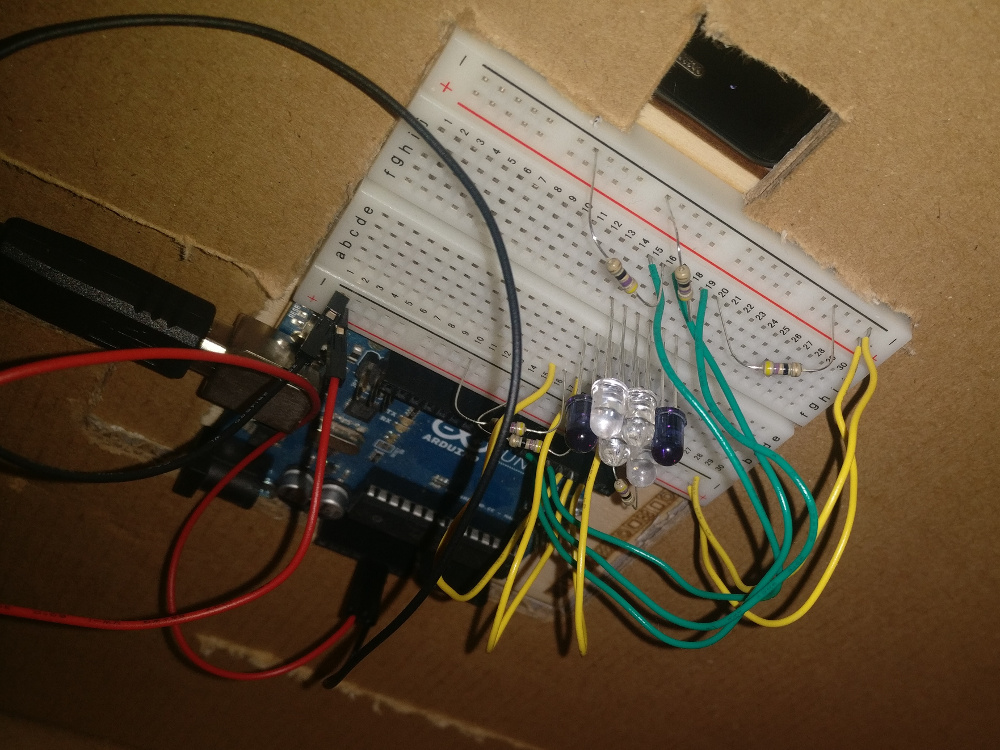
\includegraphics[height=7cm]{arduino_1}
                \label{fig:arduino_1}
            \end{figure}

            Since taking all three photos at the same time would be impossible,
            we stabilized the camera and the diodes by putting them in holes
            in a cardboard box.

            \begin{figure}[H]
                \caption{Outside view of the Arduino board and the camera.}
                \centering
                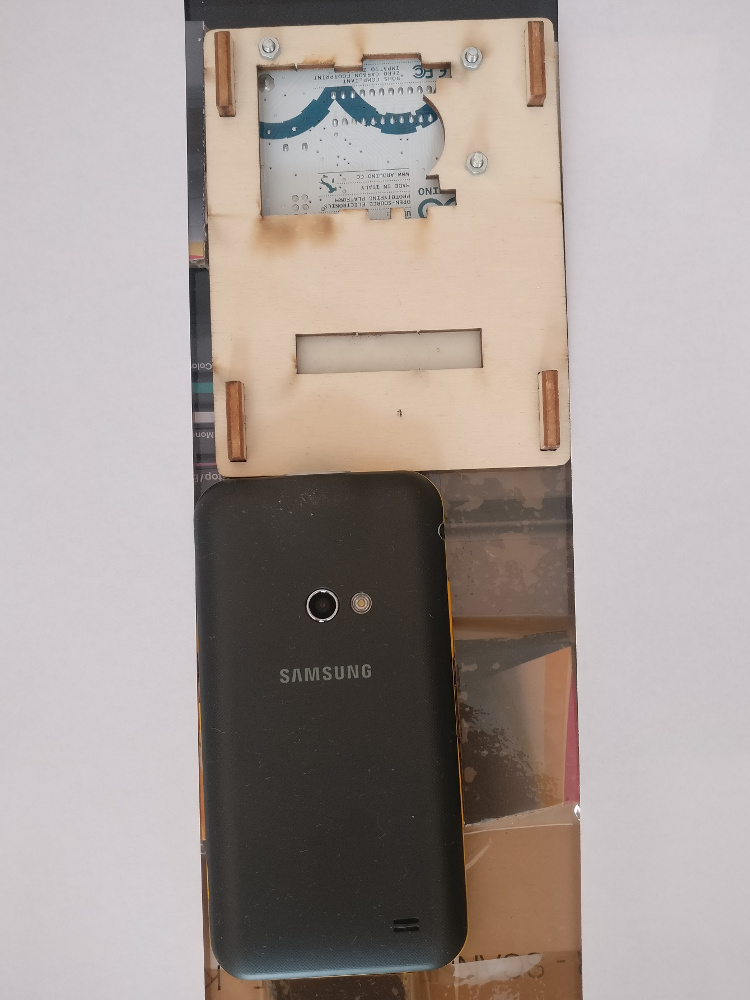
\includegraphics[height=7cm]{arduino_2}
                \label{fig:arduino_2}
            \end{figure}

            TODO

            \subsubsection*{Detecting skin}
            TODO

    \subsection{Results}
        Wide discussion about results.

    \subsection{RGB skin detection symulation}
        Using RGB to deteckt skin on picture.
        Mtoivations.

        Description of not ours solutions.

        \subsubsection*{Case-study}
            Description of problem using math.
            Final algorithm.
